\begin{frame}{Main goal}
\begin{block}{}
\begin{itemize}
\item Present a novel technique to reconstruct the \textbf{depth map} of a scene from a limited number of views. This can be applied in view synthesis and rendering for free viewpoint VR.
\begin{figure} 
\centering
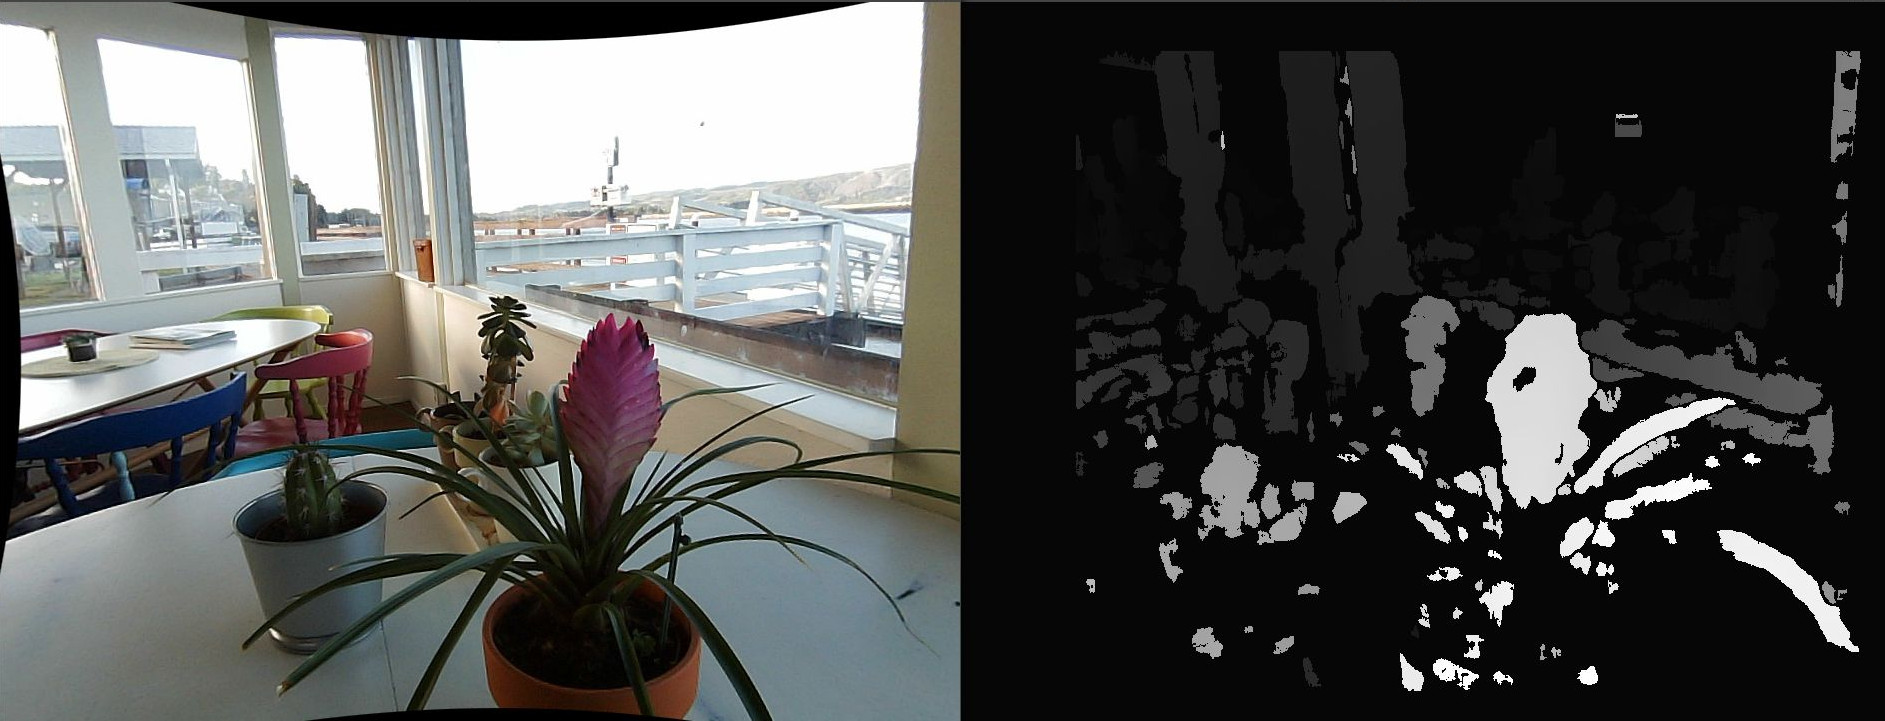
\includegraphics[width=0.8\textwidth]{./images/depth-final.jpg}
\end{figure}

\pause 
\item Explain the main building blocks of the technique: Light Field and Shearlets.

\pause
\item Show a free hardware/software implementation using julia, python and Raspberry Pi.
\end{itemize}
\end{block}
\end{frame}

\begin{frame}{What is a Light Field?}
\begin{block}{}
\begin{itemize}

\item Light can be interpreted as a field, i.e. assignment of a vector to each point in the space (M. Faraday, 1846).

\pause

\item Propagation of light rays in the 3D space is completely described by a 7D continuous function $L:\mathbb{R}^7\longrightarrow \mathbb{R}^3$, $L(x,y,z,\theta,\phi, \lambda, \tau)$ called the \textbf{plenoptic function}

\pause
\begin{figure}[h!]
\centering
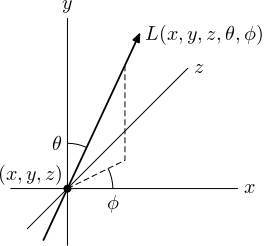
\includegraphics[width=0.3\textwidth]{./images/Plenoptic_function.jpg}
\end{figure}

\pause

\item $L$ can be simplified to a 4D function $L_4$, called \textbf{4D Light Field} or simply \textbf{Light Field}, which quantifies the intensity of static and monochromatic light rays propagating in half space. 
\end{itemize}
\end{block}
\end{frame}

\begin{frame}{4D Light Field Representation}
\begin{figure}[h!]
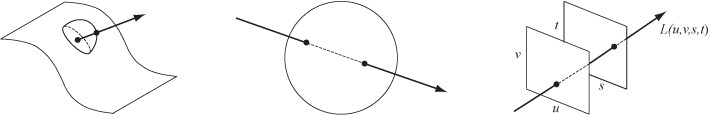
\includegraphics[width=0.8\textwidth]{./images/Light-field-parametrizations.jpg}
\caption{Three different representation of 4F LF\@. Left: $L_4(u,v,\phi,\theta)$. Center: $L_4(\phi_1,\theta_1,\phi_2,\theta_2)$. Right: $L_4(u,v,s,t)$.}
\end{figure}
\pause
\begin{figure}[h!]
\centering
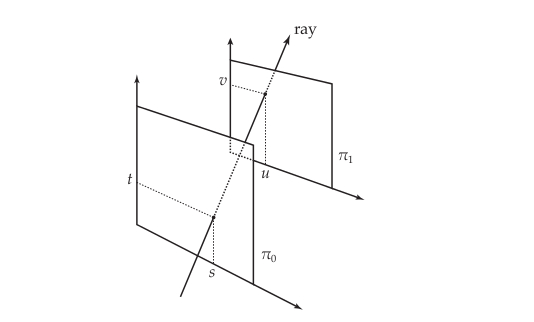
\includegraphics[width=0.5\textwidth]{./images/two-planes_param.jpg}
\caption{Used representation: "Two plane parametrization".}
\label{fig:C2S0F3}
\end{figure}
\end{frame} 

\begin{frame}{From LF to 3D}
\begin{block}{}
\begin{itemize}
\item \textbf{Stereo Vision:} The human brain generates the 3D depth perception of its sorroundings by triangulating the points of a scene using the information coming from both eyes.

\pause
\item \textbf{Epipolar Geometry:} Generalization of Stereo Vision with more than two views, assuming the epipolar constraint.

\pause
\item \textbf{Epipolar Constraint:} Analysis of object position while assuming the knowledge of the camera motion.
\end{itemize}
\end{block}
\begin{figure}[h!]
\centering
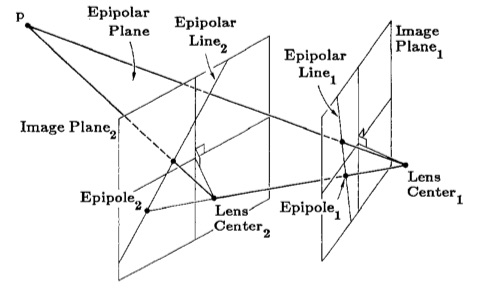
\includegraphics[width=0.52\textwidth]{./images/epipolarline.jpg}
\end{figure}
 
\end{frame}

\begin{frame}{Epipolar Plane Images (EPIs) on Straight Line Trajectories}
\begin{figure}[h!]
\centering
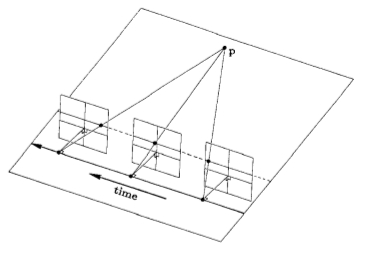
\includegraphics[width=0.45\textwidth]{./images/perp-move.jpg}
\end{figure}

\begin{figure}[h!]
\centering
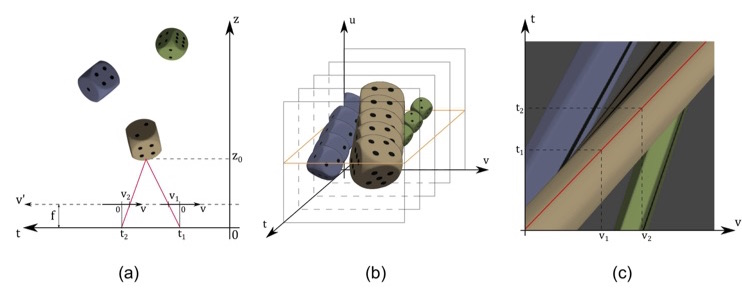
\includegraphics[width=0.90\textwidth]{./images/EPI-dices.jpg}
\end{figure}
\end{frame}


\begin{frame}{Depth map estimation with EPIs}

\begin{figure}[h!]
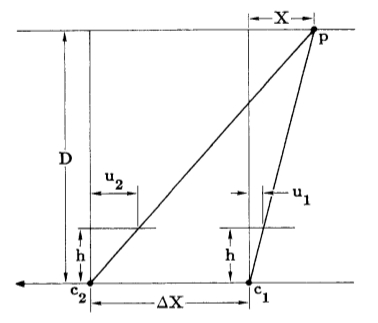
\includegraphics[width=0.5\textwidth]{./images/stereo-dist.jpg}
\end{figure}

\begin{block}{}
\begin{itemize}
\item \textbf{Point-depth formula:} $D= h\frac{\Delta X}{\Delta u}=h\frac{\Delta X}{u1-u2}$.

\item \textbf{Sampling rate (Nyquist criterion):} $\Delta X\leq \frac{D_{min}}{h}\Delta u$.

\end{itemize}
\end{block}
\end{frame}

\begin{frame}{Commercial LF (Epipolar) camera}

\begin{figure}[h!]
\centering
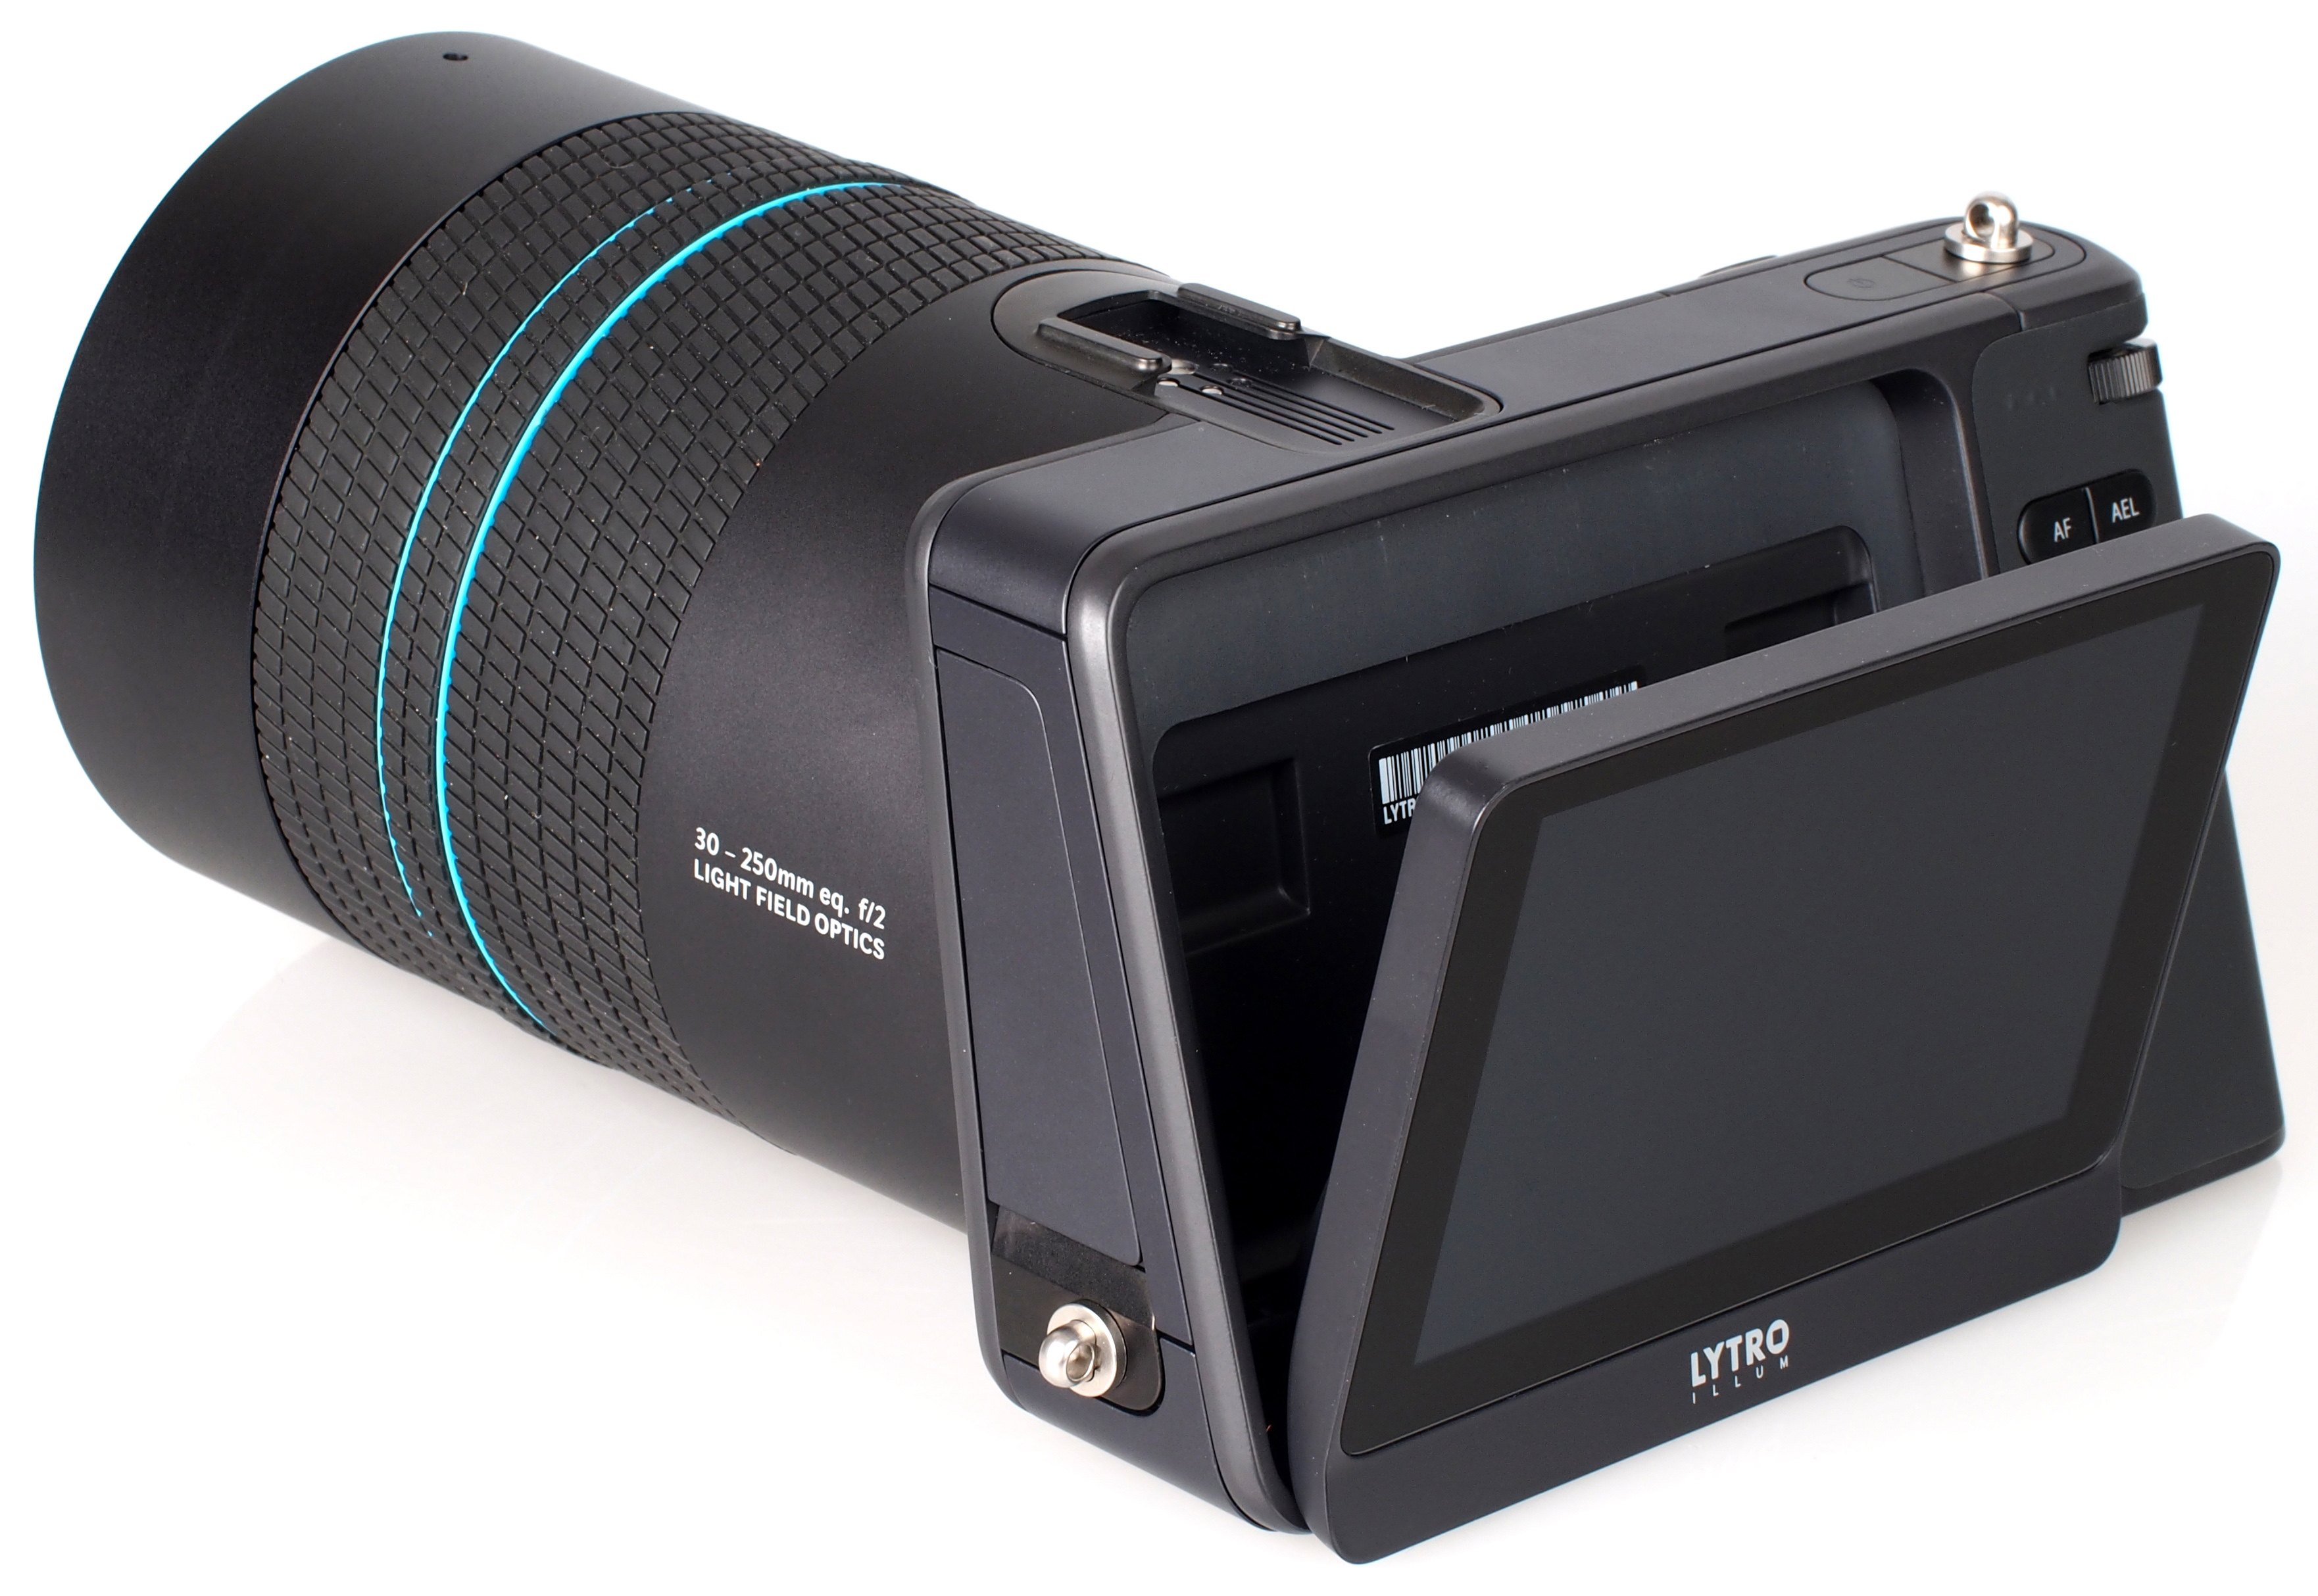
\includegraphics[width=0.45\textwidth]{./images/lytro.jpg}
\end{figure}

\begin{figure}[h!]
\centering
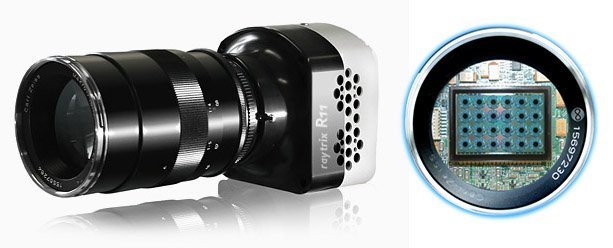
\includegraphics[width=0.90\textwidth]{./images/raytrix.jpg}
\end{figure}
\end{frame}

\begin{frame}{Our approach: Sub-Nyquist reconstruction via inpainting}

\begin{figure}[h!]
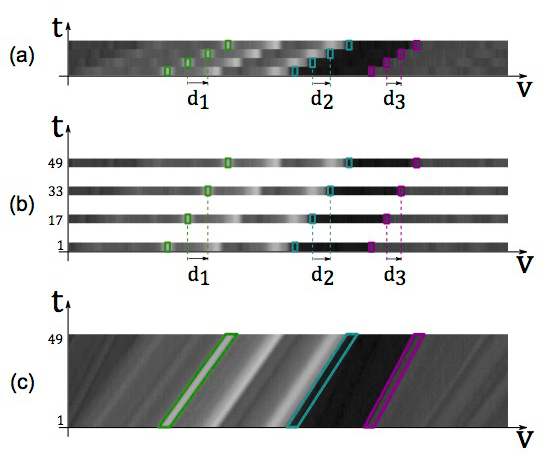
\includegraphics[width=0.7\textwidth]{./images/sparse_EPI.jpg}
\end{figure}

\end{frame}

\begin{frame}{(General) Image inpainting}
\begin{block}{\textbf{Mathematical formulation}}
 Recover an image $f\in X$ from known data:
$$
g = P_K(f)
$$
where $P_K$ is and orthogonal projection onto the known subspace $X_K\triangleleft X$.
\end{block}

\begin{figure}[h!]
\centering
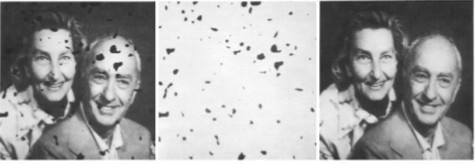
\includegraphics[width=0.9\textwidth]{./images/inpaint.jpg}
\end{figure}

\end{frame}

\begin{frame}{How to inpaint?}
\begin{block}{Frame}
A frame for a Hilbert space $X$ is a collection $\Psi=\{\psi_i\}_{i\in\mathcal{I}}\subset X$ satisfying
$$
A ||f||_2\leq ||\{\langle f,\psi_i\rangle\}_{i\in\mathcal{I}}||_{\ell^2(\mathcal{I})}\leq B||f||_2  \quad \forall f\in X
$$
for some $0<A\leq B<\infty$.
\end{block}

\bigskip

\begin{block}{\textbf{Sparse Regularization/CS approach (Genzel, Kutyniok, 2014):}}
 " If a signal (image) is sparse within a frame $\Psi$, it can be recovered from highly underdetermined, non-adaptive linear measurements by $\ell^1$-regularization, i.e.
$$
\min_{\tilde{f}\in X}||\{\langle\tilde{f},\psi_i\rangle\}_{i\in\mathcal{I}}||_{\ell^1(\mathcal{I})} \quad \text{s.t. }P_K(\tilde{f})=g=P_K(f) \quad "
$$

\end{block}

\end{frame}

\begin{frame}{Frames for images and optimal sparsity}
\begin{itemize}
\item Gabor frames (Gabor, 1946).

\bigskip
\item Wavelet frames (Morlet et al., 1984).

\bigskip
\item Curvelet frames (Cand\`es et al., 1999).

\bigskip

\item Shearlet frames (Kutyniok et al., 2005).
\end{itemize}

\pause

\begin{block}{Best N-term approx.\ error (Donoho, 2001)}
Let $\{\psi_{\lambda}\}_{\lambda\in\Lambda}\subset L^2(\mathbb{R}^2)$ a frame. The optimal best N-Term approximation error for any $f\in\mathcal{E}^2(\mathbb{R}^2)$ is
$$
\sigma_N(f,\{\psi_{\lambda}\}_{\lambda\in\Lambda})=O(N^{-1})
$$
\end{block}
\pause
\begin{block}{Error of 2D-wavelets}
$$
\sigma_N(f,\{\psi_{\lambda}\}_{\Lambda})\sim N^{-1/2}
$$
\end{block}
\end{frame}

\begin{frame}{Shearlet Transform (Kutyniok, Guo, Labate, 2005)}
\begin{block}{Classical Shearlet Transform}
$$
\langle f,\psi_{j,k,m}\rangle =\int_{\mathbb{R}^2}f(x)\overline{\psi_{j,k,m}(x)}dx
$$

where
$$
\mathcal{SH}(\psi)=\{\psi_{j,k,m}(x)=2^{3j/4}\psi (S_kA_jx-m):(j,k)\in\mathbb{Z}^2,m\in\mathbb{Z}^2\}
$$
\end{block}

\begin{figure}[h!]
\centering
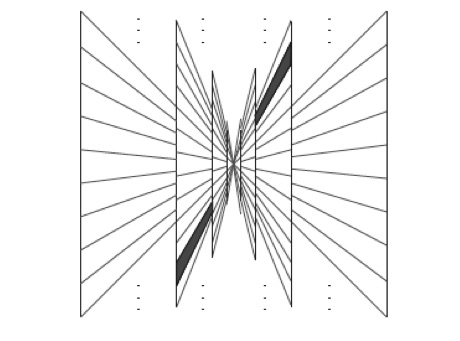
\includegraphics[width=0.4\textwidth]{./images/tiling_nocone.jpg}
\end{figure}
\end{frame}

\begin{frame}{Modification: Cone-adapted Shearlet transform}
$$
\mathcal{SH}(\phi,\psi,\tilde{\psi},c):=\mathcal{P}_{\mathcal{R}}\Phi(\phi,c1)\cup\mathcal{P}_{\mathcal{C}_1}\Psi(\psi,c)\cup\mathcal{P}_{\mathcal{C}_2}\tilde{\Psi}(\tilde{\psi,c})
$$

\begin{figure}[h!]
\centering
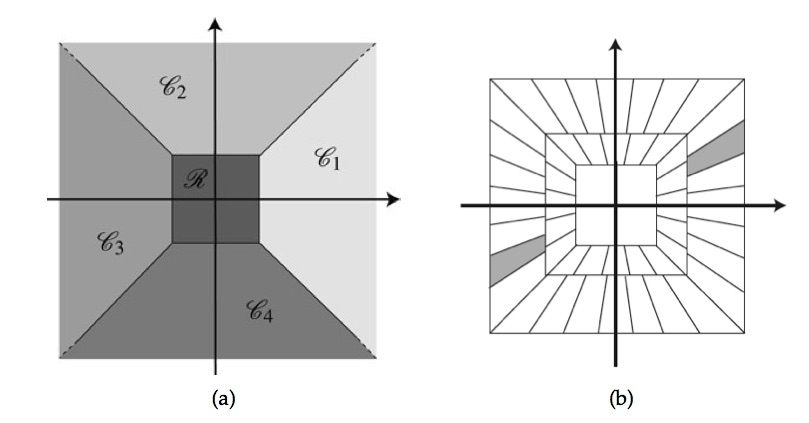
\includegraphics[width=0.6\textwidth]{./images/tiling_cone}
\end{figure}

\pause
\begin{block}{\textbf{Cone shearlets sparsity} (Band limited case: Lim, Labate; 2006), (Compactly supported case: Kutyniok, Lim, 2011)}
Best $N$-term approximation error
$$
\sigma_N(f,\{\psi_{j,k,m}\}_{j,k,m})\sim N^{-1}(\log(N))^{3/2}
$$
\end{block}
\end{frame}

\begin{frame}{Followed Pipeline}

\begin{figure}[h!]
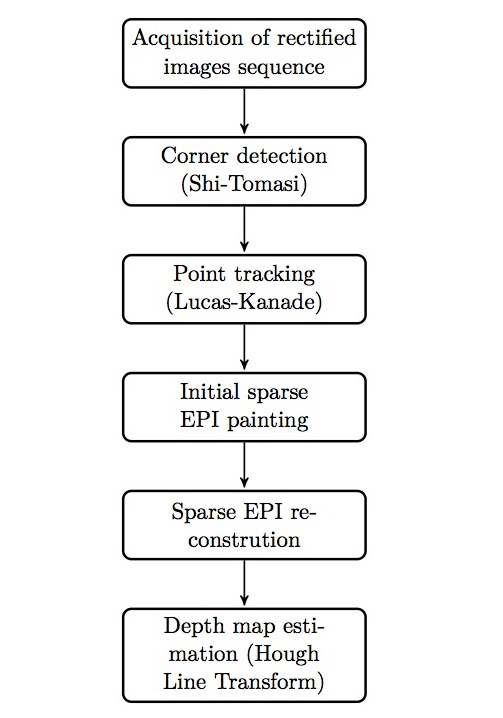
\includegraphics[width=0.47\textwidth]{./images/pipeline.jpg}
\end{figure}

\end{frame}

\begin{frame}{Physical Acquisition Setup}
\begin{block}{}
\begin{itemize}
\item \textbf{Data set:} Sequence of 101 rectified pictures of a scene generated by Professor Markus Gross' group in the Disney Research Center at Z\"urich.
\pause
\item \textbf{Technical details of physical setup:} Canon EOS 4D Mark II DSLR camera, Canon EF 50 mm f/1.4 USM lens and a Zaber T-LST1500D motorized linear stage to drive the camera to the shooting positions with 10 mm of distance between each other. 
\pause
\begin{figure}[h!]
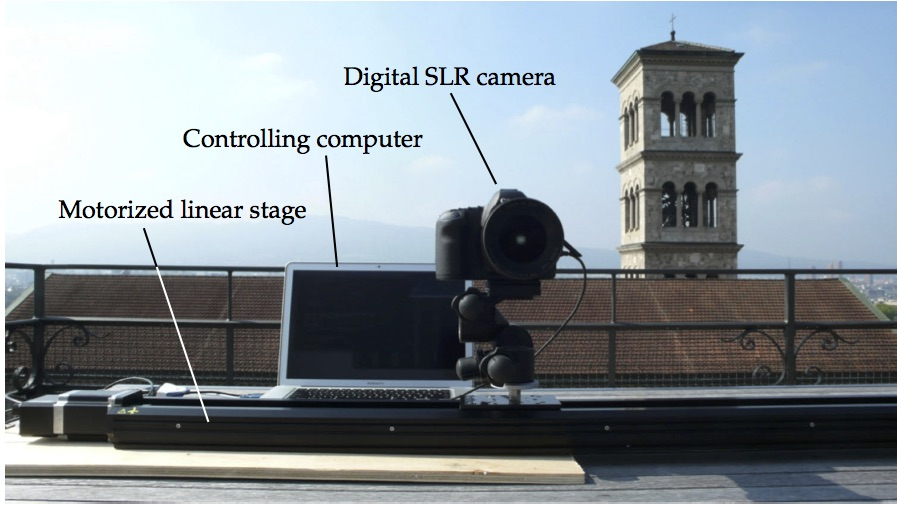
\includegraphics[width=0.6\textwidth]{./images/setting.jpg}
\end{figure}
\end{itemize}
\end{block}
\end{frame}

\begin{frame}{Used Data Set: Church}
\begin{figure}[!tbp]
  \centering
  \begin{minipage}[b]{0.49\textwidth}
    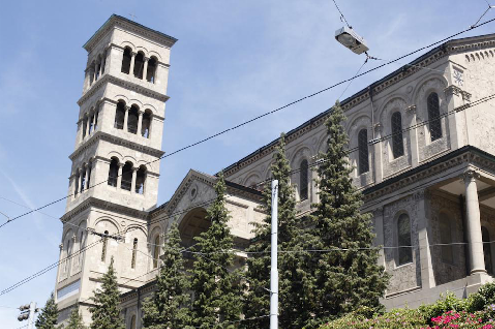
\includegraphics[width=\textwidth]{./images/first_frame_church.png}
  \end{minipage}
	\pause
 % \hfill
  \begin{minipage}[b]{0.5\textwidth}
    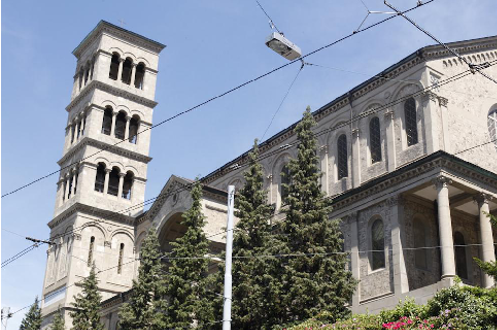
\includegraphics[width=\textwidth]{./images/last_frame_church.png}
  \end{minipage}
\end{figure}
\end{frame}

\begin{frame}{Point Tracking Results}
\begin{figure}[!tbp]
  \centering
  \begin{minipage}[b]{0.49\textwidth}
    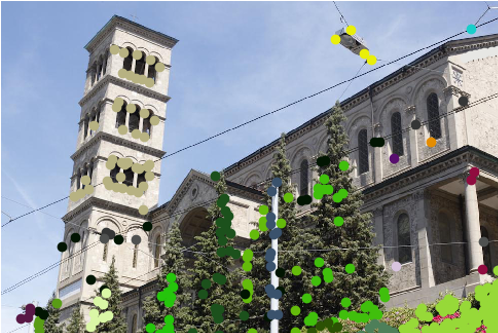
\includegraphics[width=\textwidth]{./images/first_frame_church_points.png}
  \end{minipage}
	\pause
 % \hfill
  \begin{minipage}[b]{0.5\textwidth}
    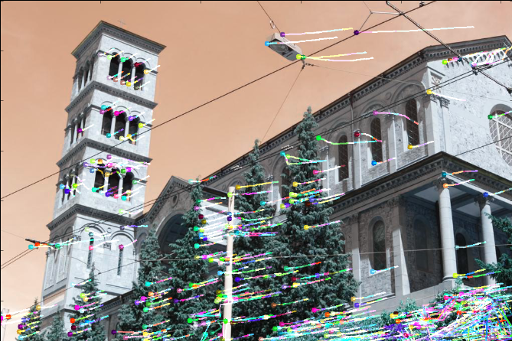
\includegraphics[width=\textwidth]{./images/track_points_church.png}
  \end{minipage}
\end{figure}
\end{frame}

\begin{frame}{Example of EPI}
\begin{figure}[h!]
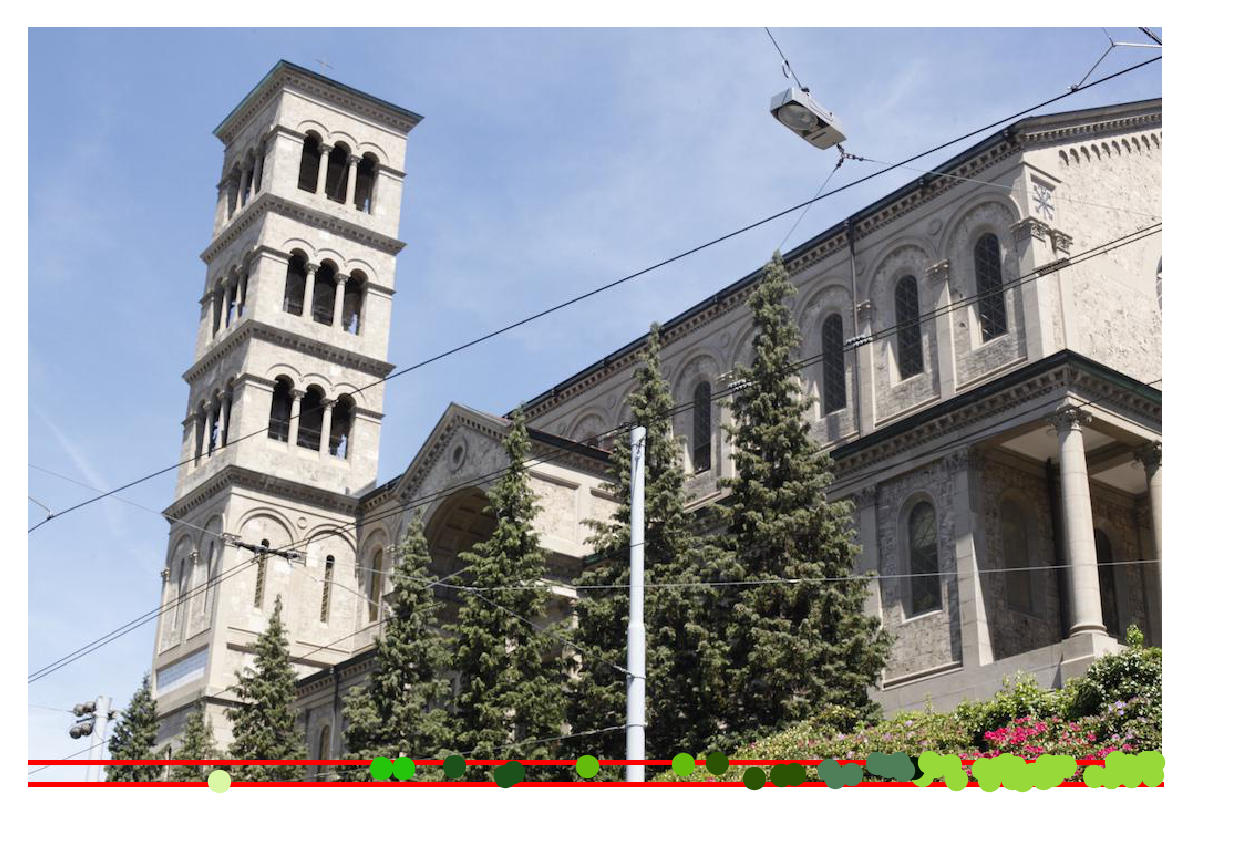
\includegraphics[width=0.45\textwidth]{./images/EPI-strip.png}
\end{figure}
\pause
\begin{figure}[!tbp]
  \centering
  \begin{minipage}[b]{0.45\textwidth}
    
\includegraphics[width=\textwidth]{./images/EPI-dense.png}
  \end{minipage}
	\pause
 % \hfill
  \begin{minipage}[b]{0.45\textwidth}
    
\includegraphics[width=\textwidth]{./images/EPI-sparse.png}
  \end{minipage}
\end{figure}

\end{frame}


\begin{frame}{Results on EPIs inpainting}
\begin{figure}[!tbp]
  \centering
  \begin{minipage}[b]{0.40\textwidth}
    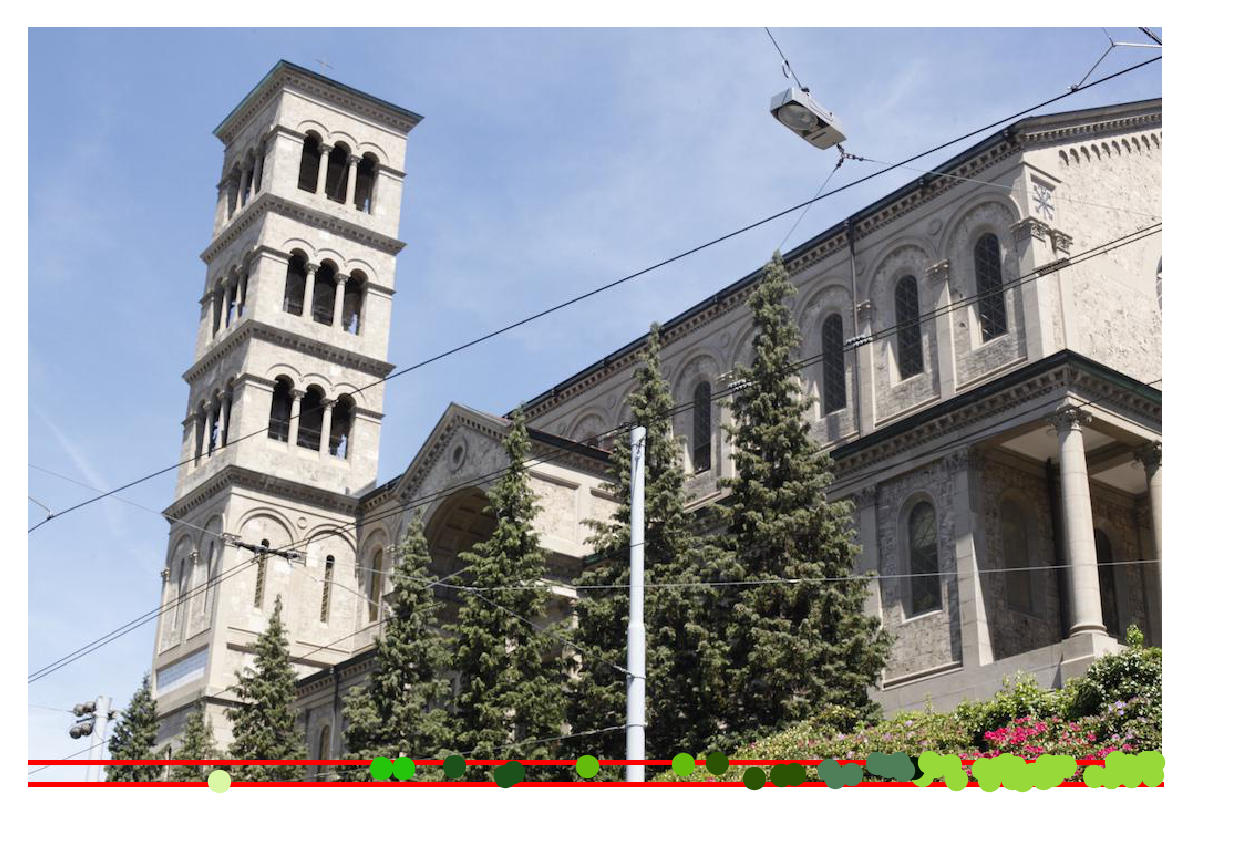
\includegraphics[width=\textwidth]{./images/EPI-strip.png}
  \end{minipage}
	\pause
 % \hfill
  \begin{minipage}[b]{0.40\textwidth}
    
\includegraphics[width=\textwidth]{./images/EPI-dense.png}
  \end{minipage}
\end{figure}
\pause

\begin{figure}[!tbp]
  \centering
  \begin{minipage}[b]{0.40\textwidth}
    
\includegraphics[width=\textwidth]{./images/EPI-sparse.png}
  \end{minipage}
	\pause
 % \hfill
  \begin{minipage}[b]{0.40\textwidth}
    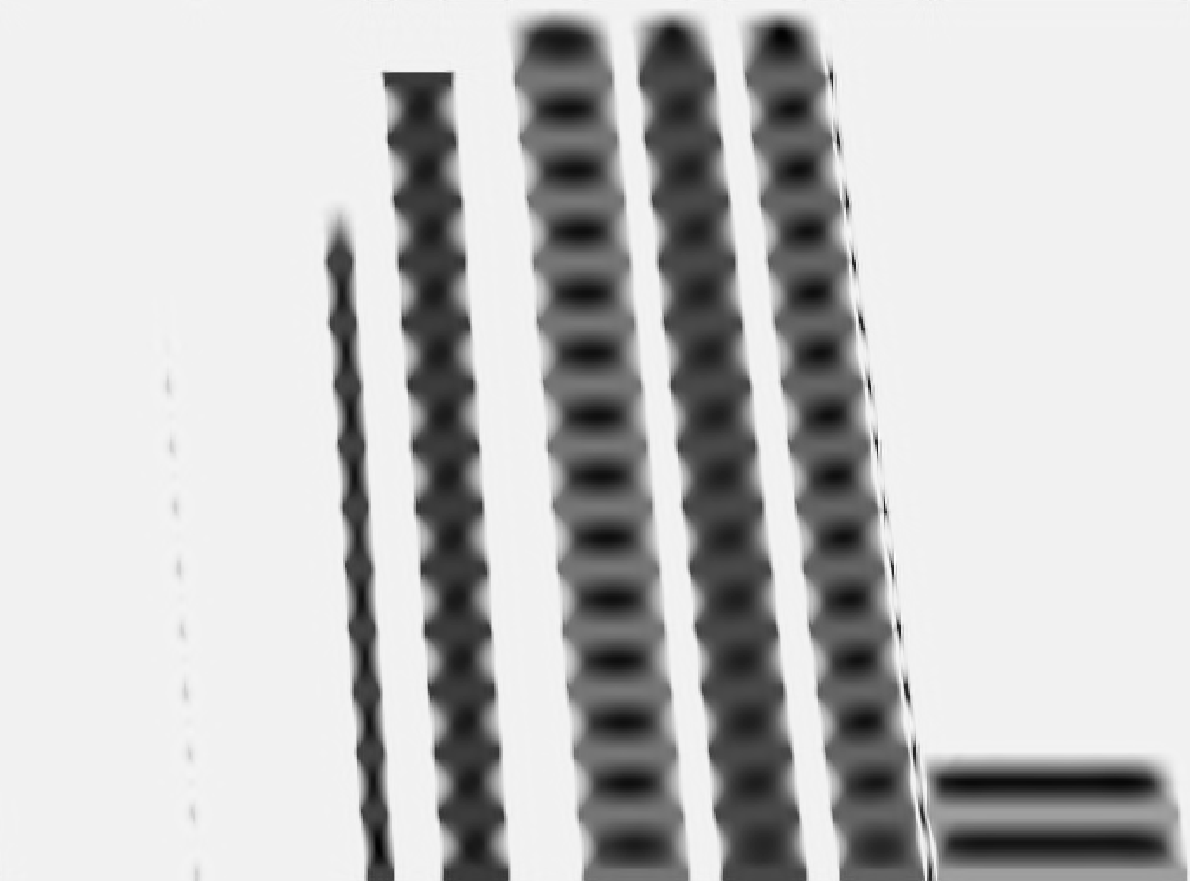
\includegraphics[width=\textwidth]{./images/EPI-inpainted.png}
  \end{minipage}
\end{figure}

\end{frame}


\begin{frame}{Results on line detection and depth map estimation}
\begin{figure}[!tbp]
  \centering
  \begin{minipage}[b]{0.40\textwidth}
    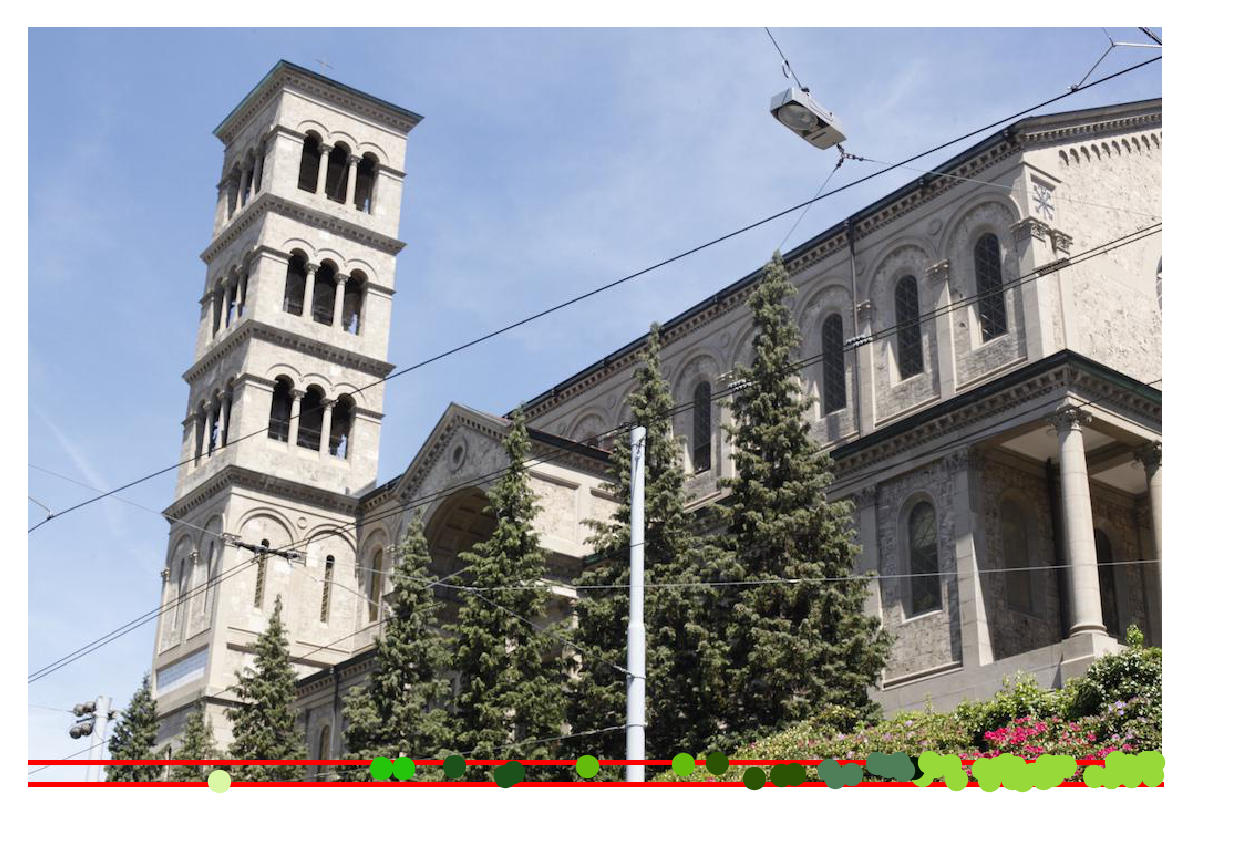
\includegraphics[width=\textwidth]{./images/EPI-strip.png}
  \end{minipage}
	\pause
 % \hfill
  \begin{minipage}[b]{0.40\textwidth}
    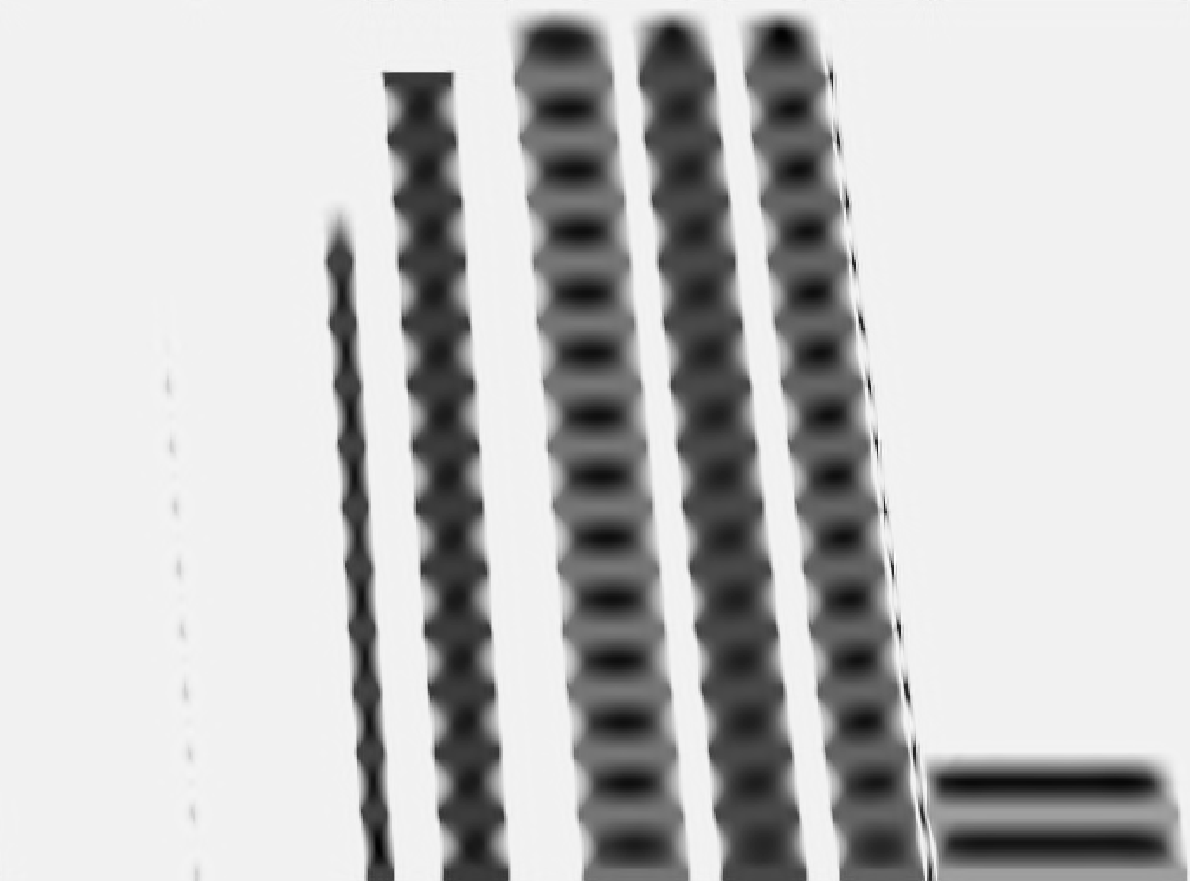
\includegraphics[width=\textwidth]{./images/EPI-inpainted.png}
  \end{minipage}
\end{figure}
\pause

\begin{figure}[!tbp]
  \centering
  \begin{minipage}[b]{0.40\textwidth}
    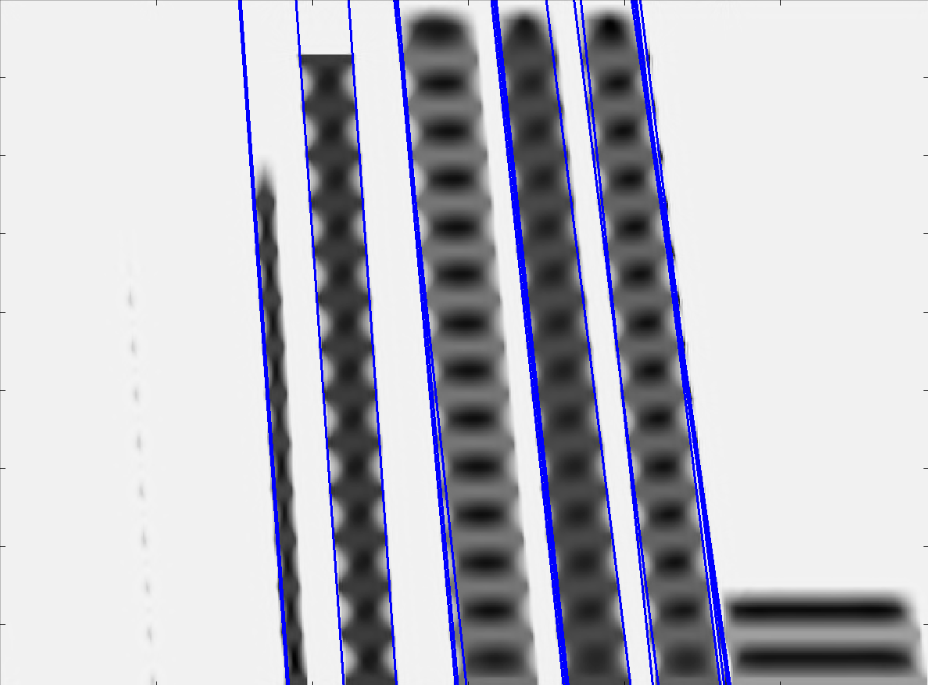
\includegraphics[width=\textwidth]{./images/EPI-lines.png}
  \end{minipage}
	\pause
 % \hfill
  \begin{minipage}[b]{0.40\textwidth}
    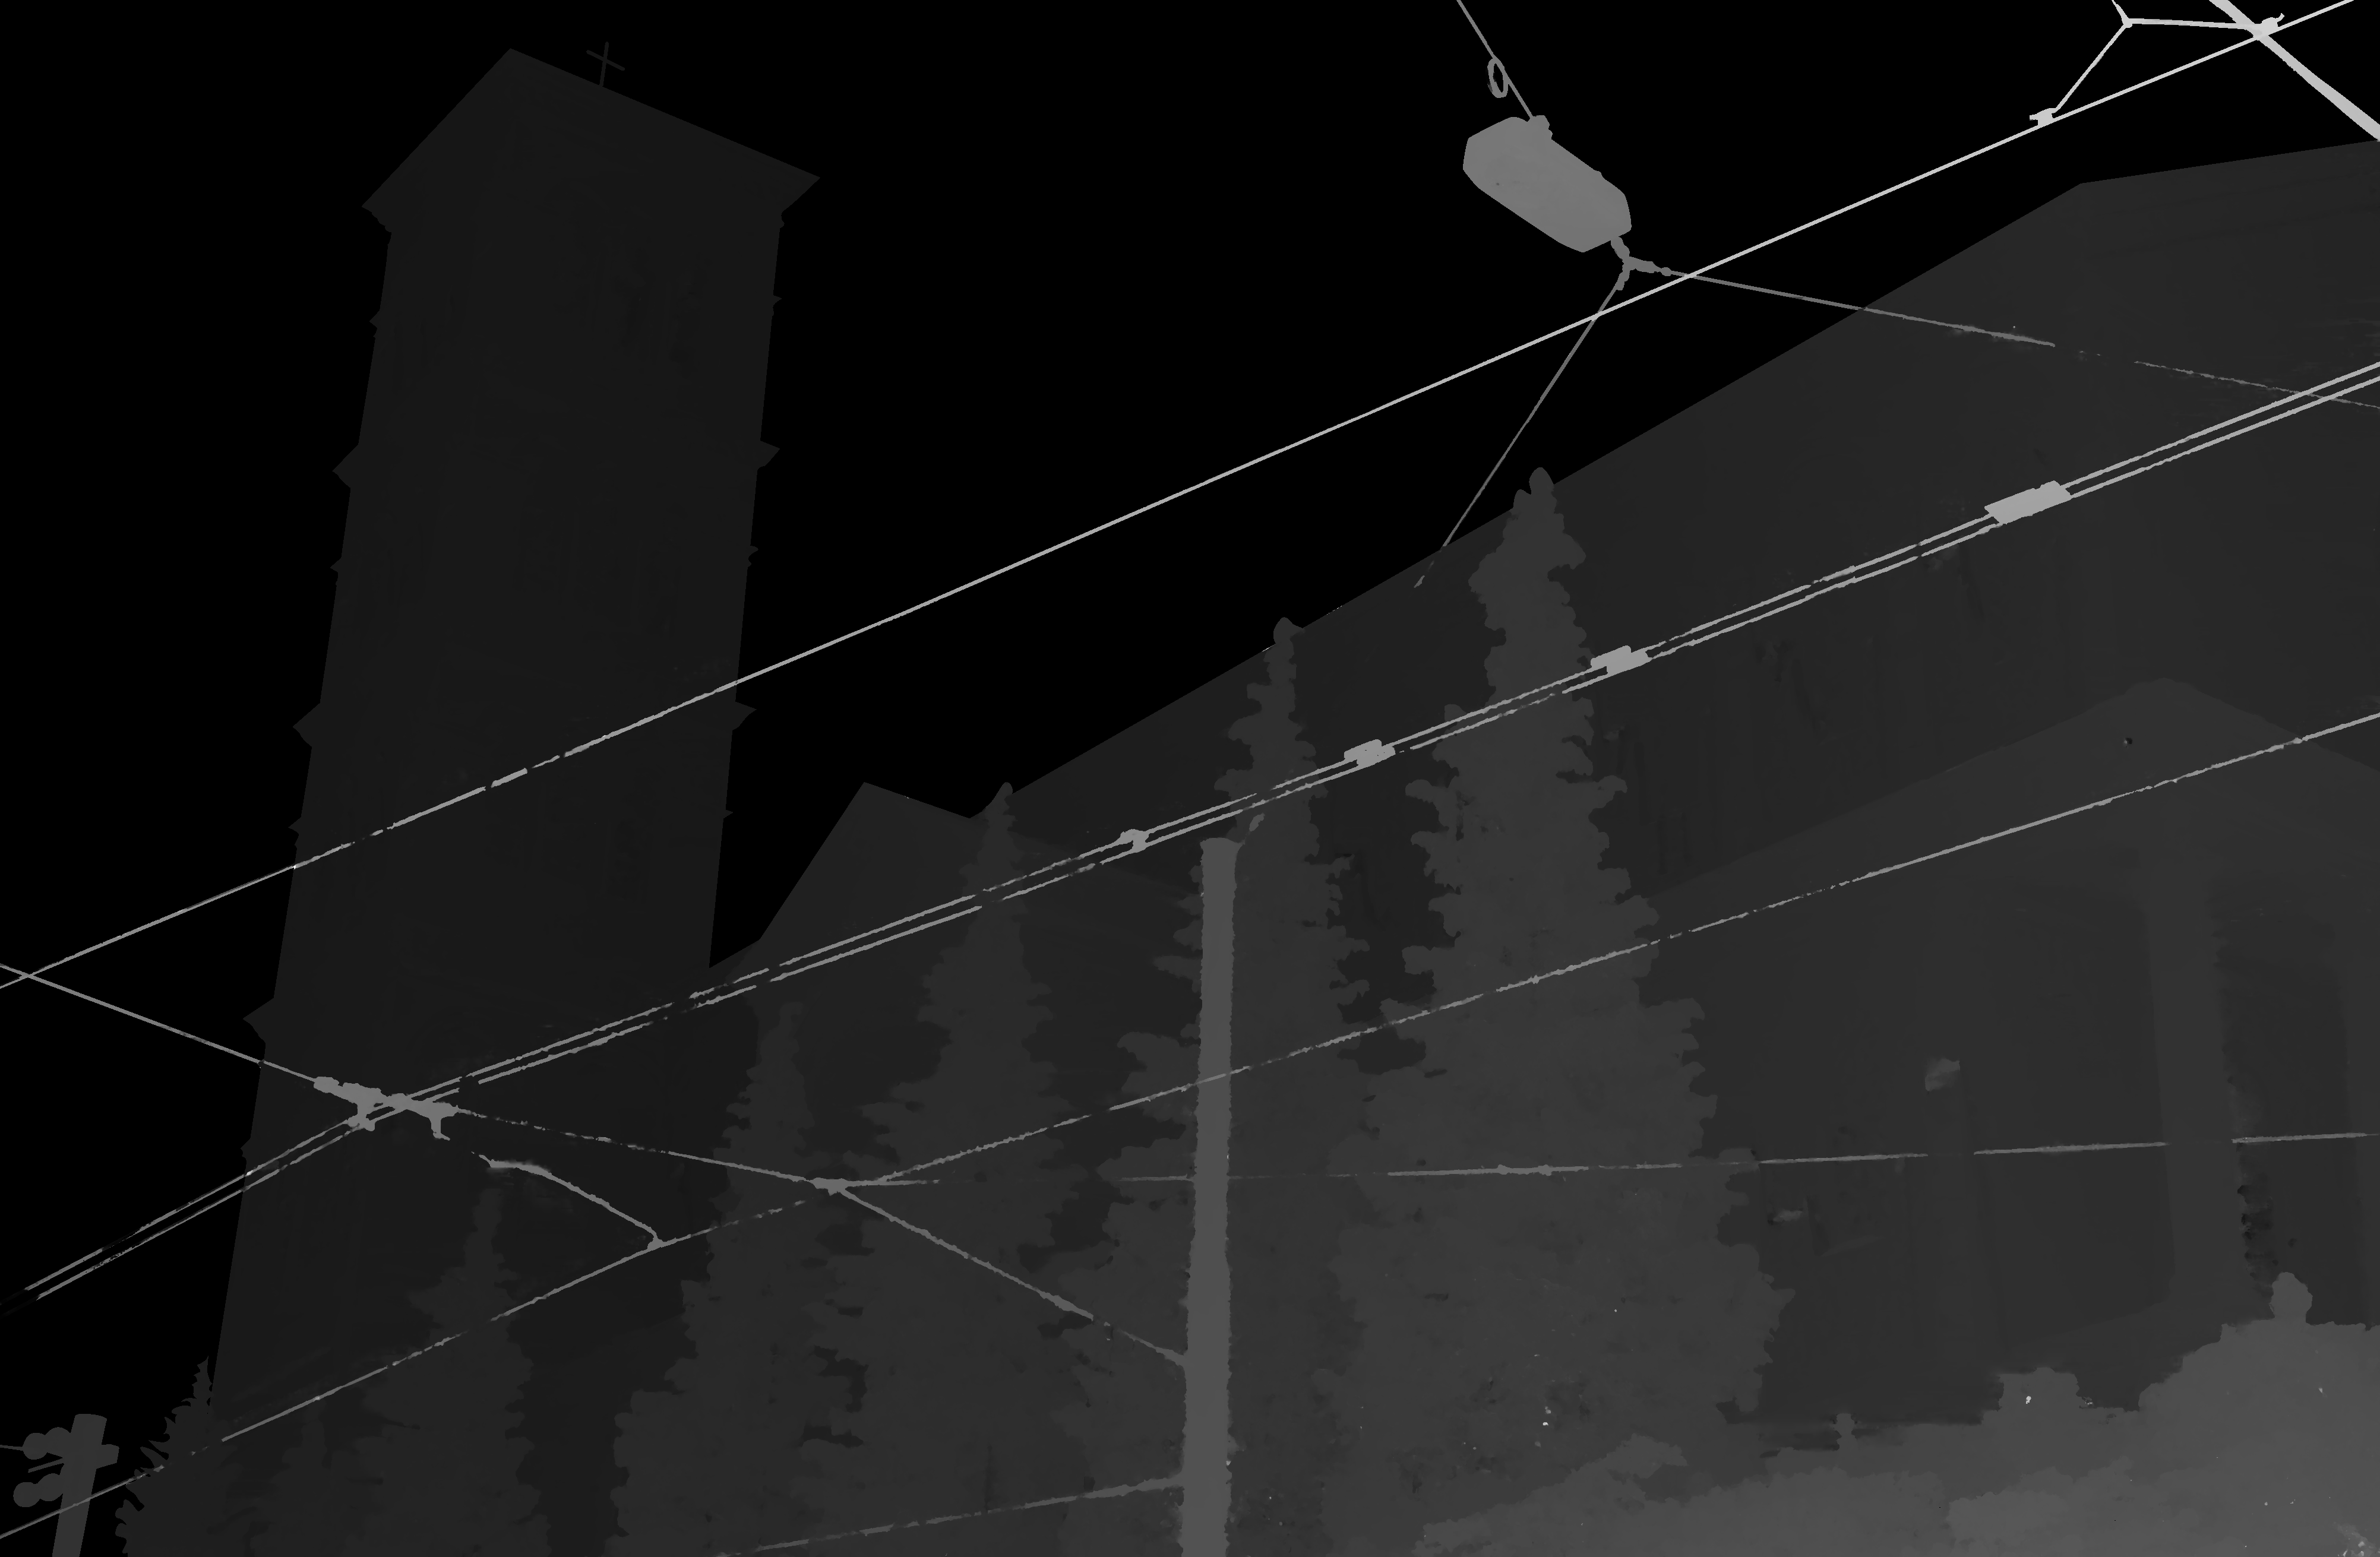
\includegraphics[width=\textwidth]{./images/dmap.png}
  \end{minipage}
\end{figure}
\end{frame}

\begin{frame}{Open Hardware Implementation}
\begin{center}
\Large{Raspberry $\pi$ + Camera module v2}
\end{center}
\begin{figure}[h!]
\centering
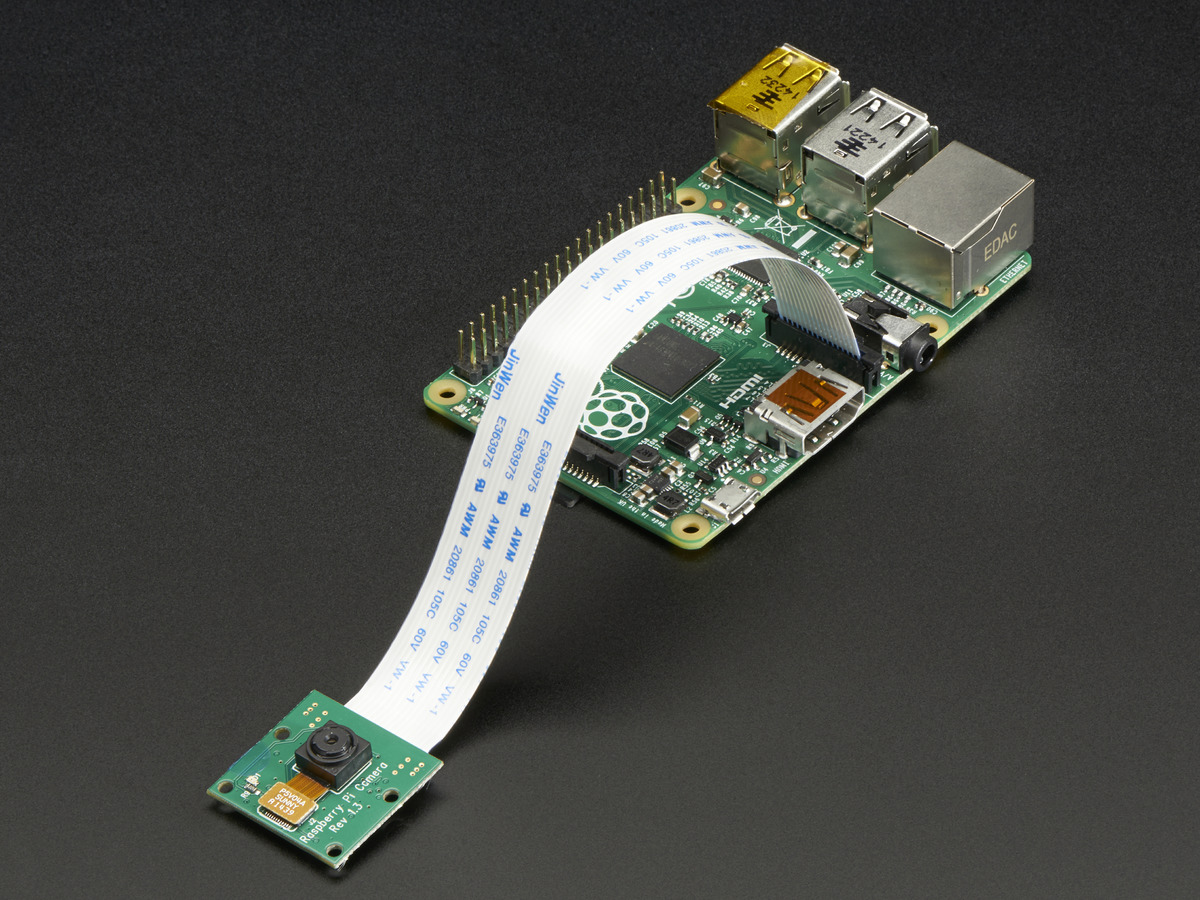
\includegraphics[width=0.78\textwidth]{./images/rpi-cam.jpg}
\end{figure}
\end{frame}

\begin{frame}{Future work}
\begin{figure}[!tbp]
  \centering
  \begin{minipage}[b]{0.49\textwidth}
    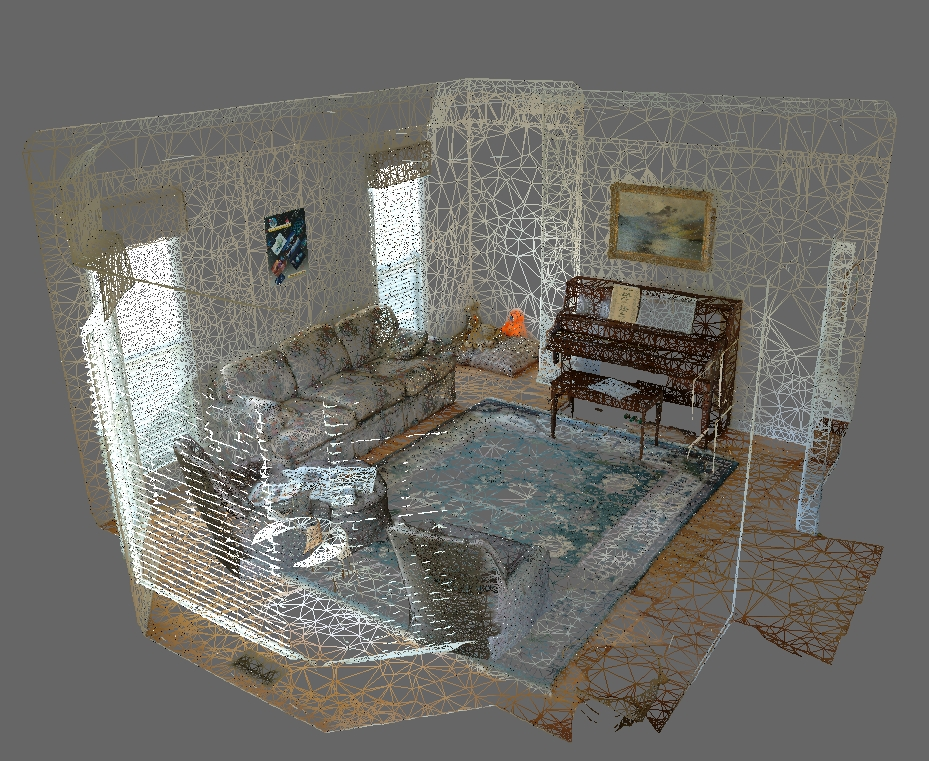
\includegraphics[width=\textwidth]{./images/livingroomwire.jpg}
  \end{minipage}
 % \hfill
  \begin{minipage}[b]{0.5\textwidth}
    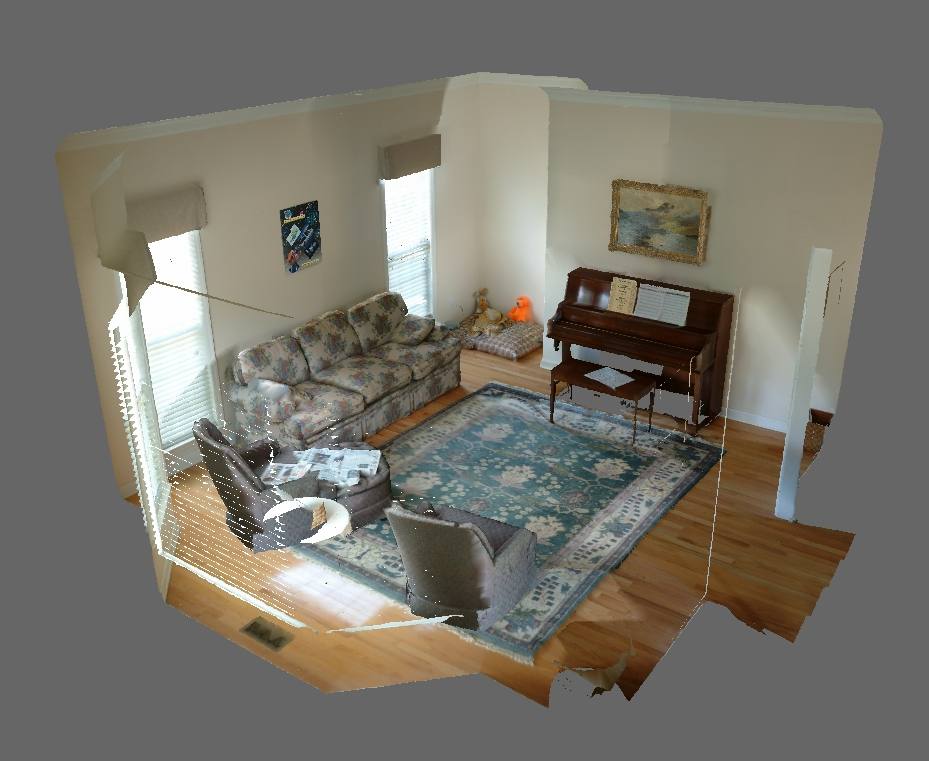
\includegraphics[width=\textwidth]{./images/backfacingoff.jpg}
  \end{minipage}
\end{figure}

\end{frame}

\begin{frame}{Thanks!}
\begin{center}
\Large{Questions?}
\end{center}
\begin{figure}[h!]
\centering
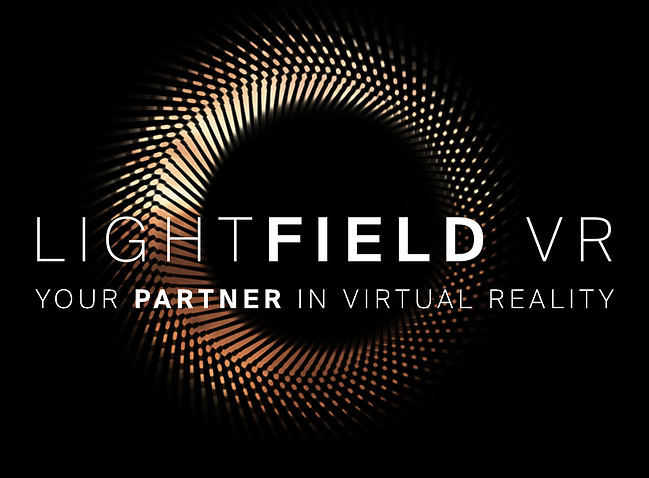
\includegraphics[width=0.8\textwidth]{./images/lf-vr.jpg}
\end{figure}
\end{frame}

